\chapter{Jeux sous forme extensive}

\section{Formalisation : Arbre et Partie}

Un jeu sous forme extensive modélise des interactions séquentielles. Il est représenté par un \textbf{arbre de jeu} $T$.

\subsection{La notion de "Partie" (Play)}
Bien qu'intuitive, la distinction entre stragégie et partie est fondamentale.
\begin{definition}[Partie]
Une \textbf{partie} (ou \textit{play}) est un chemin complet partant de la racine de l'arbre et se terminant à une feuille (nœud terminal).
\end{definition}

\begin{proposition}
Étant donné un profil de stratégies pures $x = (x_1, \dots, x_n)$, celui-ci génère une \textbf{unique partie} $\pi(x)$.
Cependant, plusieurs profils de stratégies différents peuvent générer la même partie (si leurs différences portent uniquement sur des nœuds non atteints).
\end{proposition}

\section{Représentation par Arbre (Game Tree)}

Un arbre de jeu contient :
\begin{itemize}
    \item Des \textbf{nœuds de décision} : identifient quel joueur doit jouer.
    \item Des \textbf{branches} : actions possibles à chaque nœud.
    \item Des \textbf{feuilles} : résultats et gains finaux.
\end{itemize}

\subsection{Nice Extensive Form Games}
\begin{definition}
Un "Nice Extensive Form Game" est un jeu sous forme extensive satisfaisant :
\begin{enumerate}
    \item Un arbre \textbf{fini} (horizon fini, nœuds finis, arêtes finies).
    \item À chaque nœud (sauf terminaux), il y a un \textbf{unique} joueur désigné.
    \item Aux nœuds terminaux, on a des vecteurs de gains réels (un pour chaque joueur).
\end{enumerate}
\end{definition}

\begin{exemple}[Jeu à 3 joueurs - Diagramme du cours]
\begin{center}
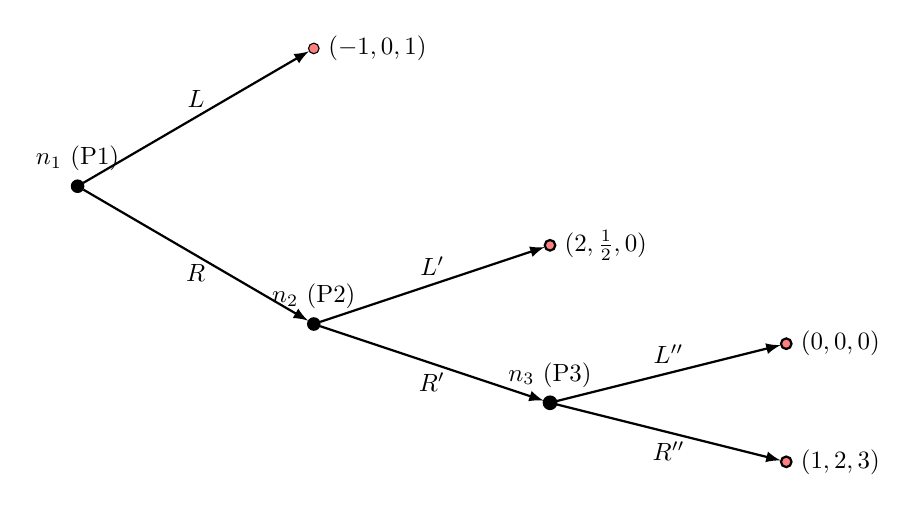
\begin{tikzpicture}[
    grow=right,
    level 1/.style={sibling distance=3.5cm,level distance=3cm},
    level 2/.style={sibling distance=2cm, level distance=3cm},
    level 3/.style={sibling distance=1.5cm, level distance=3cm},
    edge from parent/.style={draw, -latex, thick},
    every node/.style={scale=0.9},
    player/.style={circle, draw, fill=black, inner sep=1.5pt, minimum size=5pt},
    term/.style={circle, draw, fill=red!50, inner sep=1.5pt}
]
% Racine Joueur 1
\node[player, label=above:{$n_1$ (P1)}] (root) {}
    child {
        node[player, label=above:{$n_2$ (P2)}] (n2) {}
        child {
            node[player, label=above:{$n_3$ (P3)}] (n3) {}
             child {
                node[term, label=right:{$(1,2,3)$}] {}
                edge from parent node[below] {$R''$}
            }
            child {
                node[term, label=right:{$(0,0,0)$}] {}
                edge from parent node[above] {$L''$}
            }
            edge from parent node[below] {$R'$}
        }
        child {
            node[term, label=right:{$(2, \frac{1}{2}, 0)$}] {}
            edge from parent node[above] {$L'$}
        }
        edge from parent node[below] {$R$}
    }
    child {
        node[term, label=right:{$(-1, 0, 1)$}] {}
        edge from parent node[above] {$L$}
    };
\end{tikzpicture}
\end{center}
\textbf{Légende :} En noir les joueurs ($1, 2, 3$), en rouge les nœuds terminaux.
L'histoire : Joueur 1 choisit $L$ ou $R$. S'il choisit $L$, le jeu finit. S'il choisit $R$, c'est au Joueur 2, etc.
\end{exemple}

\begin{exemple}[Jeu d'entrée sur le marché]
Une firme A (Entrant) décide d'entrer (E) ou non (N). Si elle entre, la firme B (Incumbent) décide de combattre (B) ou d'accepter (A).

\begin{center}
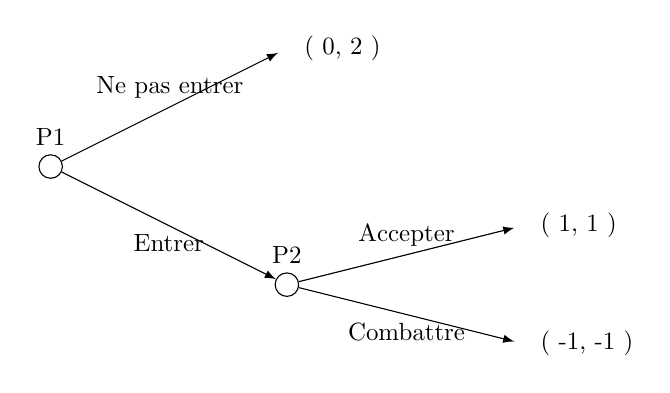
\begin{tikzpicture}[
    grow=right,
    level 1/.style={sibling distance=3cm,level distance=3cm},
    level 2/.style={sibling distance=1.5cm, level distance=3cm},
    edge from parent/.style={draw, -latex},
    every node/.style={scale=0.9}
]
\node[circle, draw, label=above:P1] (root) {}
    child {
        node[circle, draw, label=above:P2] (n1) {}
        child {
            node[label=right:{( -1, -1 )}] {}
            edge from parent node[below] {Combattre}
        }
        child {
            node[label=right:{( 1, 1 )}] {}
            edge from parent node[above] {Accepter}
        }
        edge from parent node[below] {Entrer}
    }
    child {
        node[label=right:{( 0, 2 )}] {}
        edge from parent node[above] {Ne pas entrer}
    };
\end{tikzpicture}
\end{center}
\end{exemple}

\section{Information et Stratégies}

\subsection{Information Parfaite vs Imparfaite}
\begin{itemize}
    \item \textbf{Information Parfaite :} Chaque joueur connaît l'histoire complète du jeu (tous les nœuds sont des singletons).
    \item \textbf{Information Imparfaite :} Certains nœuds sont regroupés dans des \textbf{ensembles d'information}. Le joueur sait qu'il est dans l'ensemble, mais pas à quel nœud précis.
\end{itemize}

\begin{center}
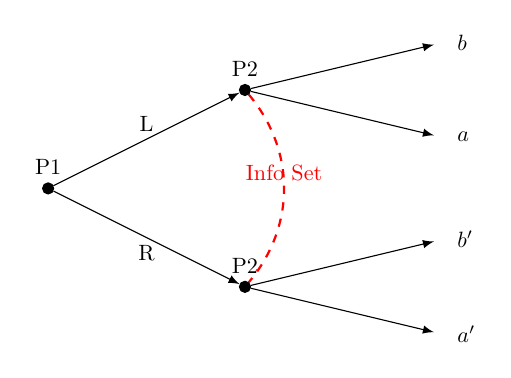
\begin{tikzpicture}[
    grow=right,
    level 1/.style={sibling distance=2.5cm,level distance=2.5cm},
    level 2/.style={sibling distance=1.2cm, level distance=2.5cm},
    edge from parent/.style={draw, -latex},
    every node/.style={scale=0.8},
    player/.style={circle, draw, fill=black, inner sep=1.5pt, minimum size=5pt}
]
% Root P1
\node[player, label=above:P1] (root) {}
    child {
        node[player, label=above:P2] (n2) {}
        child { node[label=right:{$a'$}] {} edge from parent }
        child { node[label=right:{$b'$}] {} edge from parent }
        edge from parent node[below] {R}
    }
    child {
        node[player, label=above:P2] (n1) {}
        child { node[label=right:{$a$}] {} edge from parent }
        child { node[label=right:{$b$}] {} edge from parent }
        edge from parent node[above] {L}
    };
% Information set (dashed ellipse connecting n1 and n2)
\draw[dashed, thick, red] (n1) to[bend left=40] node[midway, above, red] {Info Set} (n2);
\end{tikzpicture}
\captionof{figure}{Ensemble d'information : P2 ne sait pas si P1 a joué L ou R.}
\end{center}

\subsection{Notation Condensée des Stratégies}
Une distinction majeure du cours :
\begin{definition}[Stratégie]
Une \textbf{stratégie} est un plan d'action \textbf{complet} et \textbf{exhaustif} : elle spécifie une action pour \textit{chaque} ensemble d'information où le joueur est appelé à jouer, \textbf{même ceux qui ne seront jamais atteints} si la stratégie est suivie.
\end{definition}

\subsection{Forme Normale associée à une Forme Extensive}
\begin{definition}
À tout jeu sous forme extensive $\Gamma$, on peut associer un jeu sous forme normale (la matrice) défini par :
\begin{itemize}
    \item Les mêmes joueurs.
    \item Des stratégies définies comme des plans d'action complets (ex: $W'N'$).
    \item Des gains déterminés par la partie unique générée par chaque profil de stratégies.
\end{itemize}
\end{definition}

\begin{exemple}[Jeu "Nuclear Weapon" - Exemple du cours]
\textbf{1. Arbre du jeu ($\Gamma$) :}
Le Joueur 1 (P1) choisit Arme Nucléaire ($W$) ou Non ($N$). Le Joueur 2 (P2) réagit.
\begin{center}
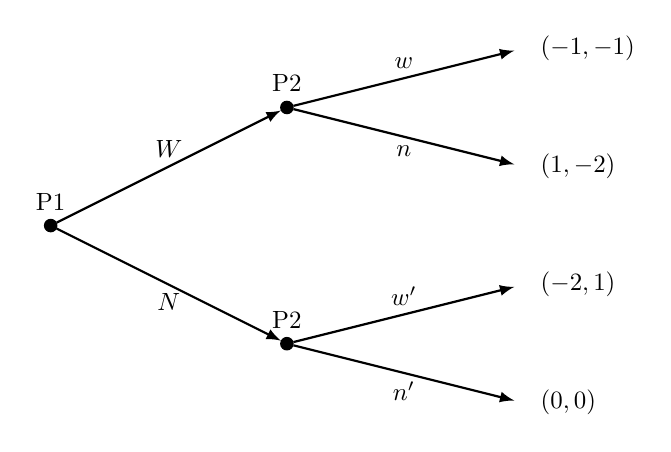
\begin{tikzpicture}[
    grow=right,
    level 1/.style={sibling distance=3cm,level distance=3cm},
    level 2/.style={sibling distance=1.5cm, level distance=3cm},
    edge from parent/.style={draw, -latex, thick},
    every node/.style={scale=0.9},
    player/.style={circle, draw, fill=black, inner sep=1.5pt, minimum size=5pt}
]
\node[player, label=above:P1] (root) {}
    child {
        node[player, label=above:P2] (n2) {}
        child {
            node[label=right:{$(0,0)$}] {}
            edge from parent node[below] {$n'$}
        }
        child {
            node[label=right:{$(-2,1)$}] {}
            edge from parent node[above] {$w'$}
        }
        edge from parent node[below] {$N$}
    }
    child {
        node[player, label=above:P2] (n1) {}
        child {
            node[label=right:{$(1,-2)$}] {}
            edge from parent node[below] {$n$}
        }
        child {
            node[label=right:{$(-1,-1)$}] {}
            edge from parent node[above] {$w$}
        }
        edge from parent node[above] {$W$}
    };
\end{tikzpicture}
\end{center}
\textit{Note : Les notations $w, n$ (gauche) et $w', n'$ (droite) pour P2 permettent de construire ses stratégies.}

\textbf{2. Stratégies :}
\begin{itemize}
    \item P1 : $\{W, N\}$
    \item P2 : $\{ww', wn', nw', nn'\}$ (Souvent noté $W'W', W'N'$ etc. dans les notes).
    Exemple : $wn'$ signifie "Je joue w si P1 joue W, et je joue n' si P1 joue N".
\end{itemize}

\textbf{3. Matrice de gains (Forme Normale) :}
Chaque case correspond au gain de la feuille atteinte.
$$
\begin{array}{c|c|c|c|c}
P1 \setminus P2 & ww' & wn' & nw' & nn' \\
\hline
W & (-1,-1) & (-1,-1) & (1,-2) & (1,-2) \\
\hline
N & (-2,1) & (0,0) & (-2,1) & (0,0) \\
\end{array}
$$
\textit{Explication :} Si P1 joue $W$ et P2 joue $wn'$, le jeu va en $W$ puis en $w$ (car la 1ère lettre de P2 est w). Le gain est $(-1,-1)$. Le choix $n'$ de P2 n'est pas observé ("counterfactual").

\textbf{4. Équilibres de Nash :}
\begin{itemize}
    \item Nash de $\Gamma$ = Nash de la forme normale.
    \item Ici, $(W, ww')$ est un Équilibre de Nash (gain $-1, -1$). Vérifiez dans la matrice.
\end{itemize}
\end{exemple}


\section{Induction Arrière et Crédibilité}

\subsection{Induction Arrière (Backward Induction)}
Pour résoudre un jeu fini à information parfaite, on raisonne à rebours :
\begin{enumerate}
    \item On se place aux derniers nœuds de décision.
    \item Le joueur choisit l'action maximisant son gain.
    \item On remplace le sous-jeu par ces gains (on "élague" l'arbre).
    \item On remonte jusqu'à la racine.
\end{enumerate}

\begin{theoreme}
L'algorithme d'induction arrière détermine un \textbf{Équilibre de Nash Parfait en Sous-Jeu (SPE)}.
\end{theoreme}

\subsection{Menaces Non Crédibles}
Tout SPE est un équilibre de Nash, mais la réciproque est fausse.
\begin{itemize}
    \item Un équilibre de Nash peut reposer sur une "menace non crédible" : le joueur promet une punition sévère (ex: se faire exploser) à un nœud qui n'est pas atteint à l'équilibre.
    \item Comme le nœud n'est jamais atteint, la menace ne coûte rien ("talk is cheap").
    \item Le concept de SPE (et l'induction arrière) élimine ces équilibres en exigeant la rationalité \textbf{partout}, même hors du chemin d'équilibre.
\end{itemize}

\section{Cas Pratique : Le Jeu du Mille-pattes (Centipede Game)}
...

\section{Exercices}
\subsection{Exercice "Arbre et Matrice" (Notes manuscrites)}
Soit le jeu suivant : P1 choisit $a$ ou $b$. P2 choisit ensuite ( $c,d$ si $a$ ; $c',d'$ si $b$).
\begin{center}
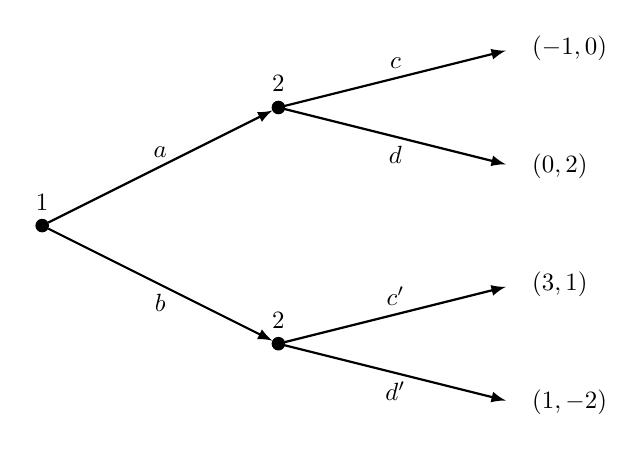
\begin{tikzpicture}[
    grow=right,
    level 1/.style={sibling distance=3cm,level distance=3cm},
    level 2/.style={sibling distance=1.5cm, level distance=3cm},
    edge from parent/.style={draw, -latex, thick},
    every node/.style={scale=0.9},
    player/.style={circle, draw, fill=black, inner sep=1.5pt, minimum size=5pt}
]
\node[player, label=above:1] (root) {}
    child {
        node[player, label=above:2] (n2) {}
        child {
            node[label=right:{$(1,-2)$}] {}
            edge from parent node[below] {$d'$}
        }
        child {
            node[label=right:{$(3,1)$}] {}
            edge from parent node[above] {$c'$}
        }
        edge from parent node[below] {$b$}
    }
    child {
        node[player, label=above:2] (n1) {}
        child {
            node[label=right:{$(0,2)$}] {}
            edge from parent node[below] {$d$}
        }
        child {
            node[label=right:{$(-1,0)$}] {}
            edge from parent node[above] {$c$}
        }
        edge from parent node[above] {$a$}
    };
\end{tikzpicture}
\end{center}
\textbf{Question :} Calculer les équilibres de Nash.
\\
\textbf{Réponse :}
On construit la matrice $2 \times 4$. Stratégies P2 : $cc', cd', dc', dd'$.
$$
\begin{array}{c|c|c|c|c}
1 \setminus 2 & cc' & cd' & dc' & dd' \\
\hline
a & (-1,0) & (-1,0) & \mathbf{(0,2)} & \mathbf{(0,2)} \\
\hline
b & \mathbf{(3,1)} & (1,-2) & \mathbf{(3,1)} & (1,-2) \\
\end{array}
$$
\begin{itemize}
    \item Si P1 joue $a$ : P2 préfère $d$ (gain 2) $\to$ colonnes $dc', dd'$. P1 répond $a$ ou $b$ ? Comparons $0$ et $3$. P1 préfère $b$. Donc pas de Nash pure sur la ligne $a$.
    \item Si P1 joue $b$ : P2 préfère $c'$ (gain 1) $\to$ colonnes $cc', dc'$. P1 répond $b$ (3 vs -1 ou 0).
    \item \textbf{Nash Equilibria :} $(b, cc')$ et $(b, dc')$.
    \item Gain à l'équilibre : $(3,1)$.
\end{itemize}
\section{Induction Arrière et Crédibilité}

\subsection{Induction Arrière (Backward Induction)}
Pour résoudre un jeu fini à information parfaite, on raisonne à rebours :
\begin{enumerate}
    \item On se place aux derniers nœuds de décision.
    \item Le joueur choisit l'action maximisant son gain.
    \item On remplace le sous-jeu par ces gains (on "élague" l'arbre).
    \item On remonte jusqu'à la racine.
\end{enumerate}

\begin{theoreme}
L'algorithme d'induction arrière détermine un \textbf{Équilibre de Nash Parfait en Sous-Jeu (SPE)}.
\end{theoreme}

\subsection{Menaces Non Crédibles}
Tout SPE est un équilibre de Nash, mais la réciproque est fausse.
\begin{itemize}
    \item Un équilibre de Nash peut reposer sur une "menace non crédible" : le joueur promet une punition sévère (ex: se faire exploser) à un nœud qui n'est pas atteint à l'équilibre.
    \item Comme le nœud n'est jamais atteint, la menace ne coûte rien ("talk is cheap").
    \item Le concept de SPE (et l'induction arrière) élimine ces équilibres en exigeant la rationalité \textbf{partout}, même hors du chemin d'équilibre.
\end{itemize}

\section{Cas Pratique : Le Jeu du Mille-pattes (Centipede Game)}

\textbf{Description :}
Deux joueurs alternent. À chaque tour, un joueur peut "Arrêter" (Stop) et prendre le gros lot (laissant peu à l'autre), ou "Continuer" (Pass) pour augmenter la cagnotte globale.
Le jeu a une fin fixe (ex: 100 tours).

\textbf{Paradoxe de l'Induction Arrière :}
\begin{itemize}
    \item Au dernier tour (100), le joueur décideur a intérêt à Arrêter pour prendre le gain.
    \item Anticipant cela, au tour 99, l'autre joueur a intérêt à Arrêter pour ne pas se faire avoir au tour 100.
    \item Par récurrence, l'induction arrière prédit que \textbf{le premier joueur arrête dès le premier tour} !
\end{itemize}
\textbf{Conclusion :} Bien que rationnel au sens SPE, ce résultat est sous-optimal (Pareto-inférieur à la coopération) et rarement observé en pratique.

\section{Exercices}
\begin{exercice}[Jeux en Forme Extensive]
\begin{itemize}
    \item Représenter le Dilemme du Prisonnier séquentiel.
    \item Vérifier que dans le jeu d'entrée, la menace "Combattre" n'est pas crédible si le coût du combat est trop élevé.
\end{itemize}

\paragraph{Correction :}
\begin{enumerate}
    \item \textbf{PD Séquentiel :}
    J1 joue (C ou D). Puis J2 joue (C ou D) en connaissant le choix de J1.
    
    \begin{center}
    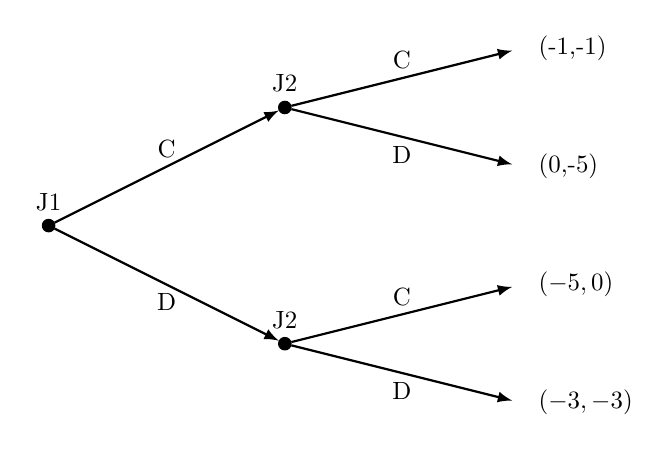
\begin{tikzpicture}[
        grow=right,
        level 1/.style={sibling distance=3cm,level distance=3cm},
        level 2/.style={sibling distance=1.5cm, level distance=3cm},
        edge from parent/.style={draw, -latex, thick},
        every node/.style={scale=0.9},
        player/.style={circle, draw, fill=black, inner sep=1.5pt, minimum size=5pt}
    ]
    \node[player, label=above:J1] (root) {}
        child {
            node[player, label=above:J2] (n2) {}
            child {
                node[label=right:{$(-3,-3)$}] {}
                edge from parent node[below] {D}
            }
            child {
                node[label=right:{$(-5,0)$}] {}
                edge from parent node[above] {C}
            }
            edge from parent node[below] {D}
        }
        child {
            node[player, label=above:J2] (n1) {}
            child {
                node[label=right:{(0,-5)}] {}
                edge from parent node[below] {D}
            }
            child {
                node[label=right:{(-1,-1)}] {}
                edge from parent node[above] {C}
            }
            edge from parent node[above] {C}
        };
    \end{tikzpicture}
    \end{center}
    
    \textbf{Induction Arrière :}
    \begin{itemize}
        \item En haut (si J1 joue C) : J2 choisit D ($0 > -1$).
        \item En bas (si J1 joue D) : J2 choisit D ($-3 > -5$).
        \item J1 anticipe que C mène à $(0, -5)$ (pour J2 c'est le gain 0, pour J1 c'est -5 ?) \textit{Attention aux gains (J1, J2)}.
        \item Vérifions les gains :
        Si (C, C) $\to (-1, -1)$.
        Si (C, D) $\to (-5, 0)$. J2 gagne 0.
        Si (D, C) $\to (0, -5)$. J2 gagne -5.
        Si (D, D) $\to (-3, -3)$.
        \item \textbf{Nœud J2 (Haut, après C) :} J2 compare C (-1) et D (0). Il choisit D.
        \item \textbf{Nœud J2 (Bas, après D) :} J2 compare C (-5) et D (-3). Il choisit D.
        \item \textbf{Racine J1 :} Anticipe (C $\to$ J2 joue D $\to$ Gain J1 = -5) et (D $\to$ J2 joue D $\to$ Gain J1 = -3).
        \item J1 compare -5 et -3. Il choisit D.
        \item \textbf{Résultat :} (D, D).
    \end{itemize}
    
    \item \textbf{Jeu d'entrée :}
    Si l'Entrant entre, l'Incumbent a le choix entre "Se battre" (Gains : -1, -1) ou "Accepter" (Gains : 1, 1).
    Comme $1 > -1$, l'Incumbent rationnel choisira \textbf{toujours} d'Accepter.
    Toute stratégie où il menace de se battre est non crédible (ne résiste pas à l'induction arrière).
    L'Entrant le sait, donc il Entre (car $1 > 0$).
\end{enumerate}
\end{exercice}
